\documentclass[]{article}
\usepackage{lmodern}
\usepackage{amssymb,amsmath}
\usepackage{ifxetex,ifluatex}
\usepackage{fixltx2e} % provides \textsubscript
\ifnum 0\ifxetex 1\fi\ifluatex 1\fi=0 % if pdftex
  \usepackage[T1]{fontenc}
  \usepackage[utf8]{inputenc}
\else % if luatex or xelatex
  \ifxetex
    \usepackage{mathspec}
    \usepackage{xltxtra,xunicode}
  \else
    \usepackage{fontspec}
  \fi
  \defaultfontfeatures{Mapping=tex-text,Scale=MatchLowercase}
  \newcommand{\euro}{€}
\fi
% use upquote if available, for straight quotes in verbatim environments
\IfFileExists{upquote.sty}{\usepackage{upquote}}{}
% use microtype if available
\IfFileExists{microtype.sty}{%
\usepackage{microtype}
\UseMicrotypeSet[protrusion]{basicmath} % disable protrusion for tt fonts
}{}
\usepackage[margin=1in]{geometry}
\usepackage{graphicx}
\makeatletter
\def\maxwidth{\ifdim\Gin@nat@width>\linewidth\linewidth\else\Gin@nat@width\fi}
\def\maxheight{\ifdim\Gin@nat@height>\textheight\textheight\else\Gin@nat@height\fi}
\makeatother
% Scale images if necessary, so that they will not overflow the page
% margins by default, and it is still possible to overwrite the defaults
% using explicit options in \includegraphics[width, height, ...]{}
\setkeys{Gin}{width=\maxwidth,height=\maxheight,keepaspectratio}
\ifxetex
  \usepackage[setpagesize=false, % page size defined by xetex
              unicode=false, % unicode breaks when used with xetex
              xetex]{hyperref}
\else
  \usepackage[unicode=true]{hyperref}
\fi
\hypersetup{breaklinks=true,
            bookmarks=true,
            pdfauthor={Eric D. Johnson},
            pdftitle={SWC Seminar Series Final Project},
            colorlinks=true,
            citecolor=blue,
            urlcolor=blue,
            linkcolor=magenta,
            pdfborder={0 0 0}}
\urlstyle{same}  % don't use monospace font for urls
\setlength{\parindent}{0pt}
\setlength{\parskip}{6pt plus 2pt minus 1pt}
\setlength{\emergencystretch}{3em}  % prevent overfull lines
\setcounter{secnumdepth}{0}

%%% Use protect on footnotes to avoid problems with footnotes in titles
\let\rmarkdownfootnote\footnote%
\def\footnote{\protect\rmarkdownfootnote}

%%% Change title format to be more compact
\usepackage{titling}
\setlength{\droptitle}{-2em}
  \title{SWC Seminar Series Final Project}
  \pretitle{\vspace{\droptitle}\centering\huge}
  \posttitle{\par}
  \author{Eric D. Johnson}
  \preauthor{\centering\large\emph}
  \postauthor{\par}
  \predate{\centering\large\emph}
  \postdate{\par}
  \date{Thursday, March 19, 2015}




\begin{document}

\maketitle


This is a simple analysis of some gapminder data for the SWC final
project.

Look at this great Afghanistan data! The trend is all wack!

\begin{verbatim}
## [1] TRUE
\end{verbatim}

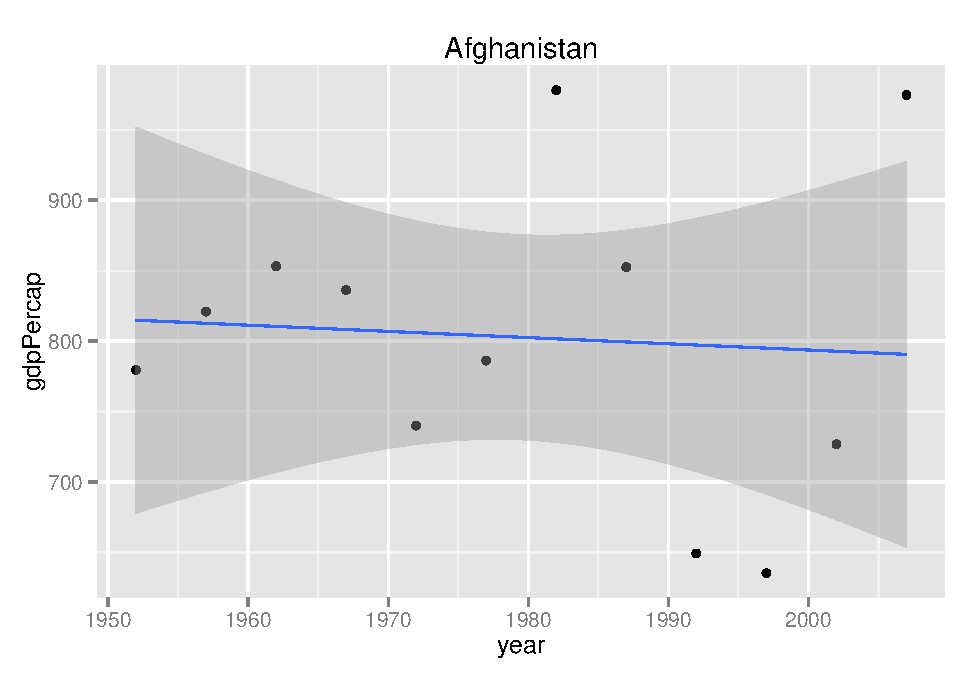
\includegraphics{GapMinder_rMarkdown_files/figure-latex/unnamed-chunk-1.pdf}

Look at this great United States data; the trend is bomb-diggity!

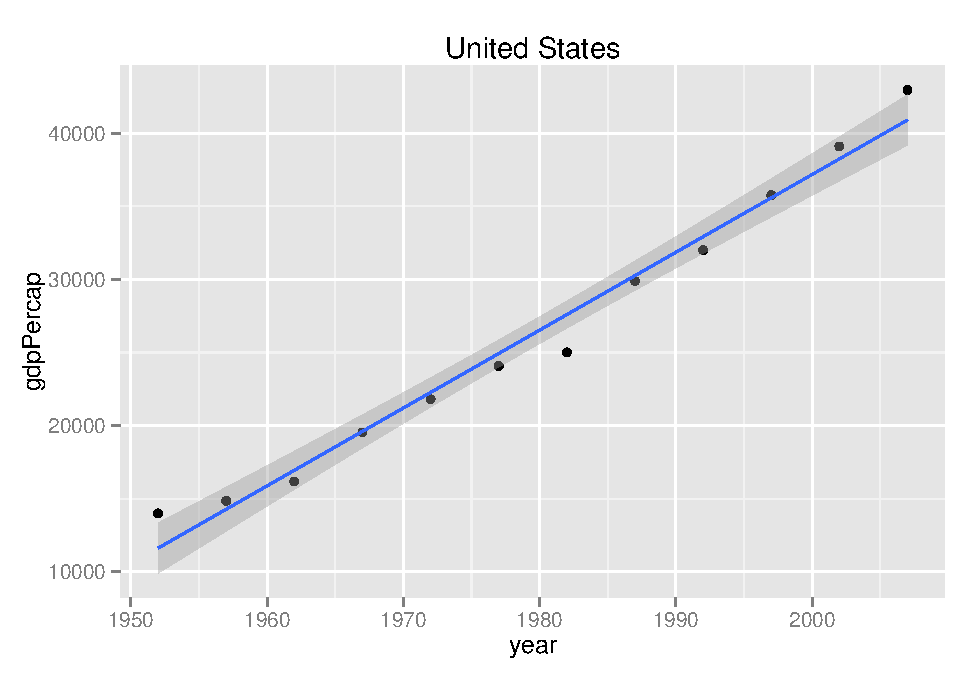
\includegraphics{GapMinder_rMarkdown_files/figure-latex/unnamed-chunk-2.pdf}

Look at this great Zimbabwe data; super gnar!

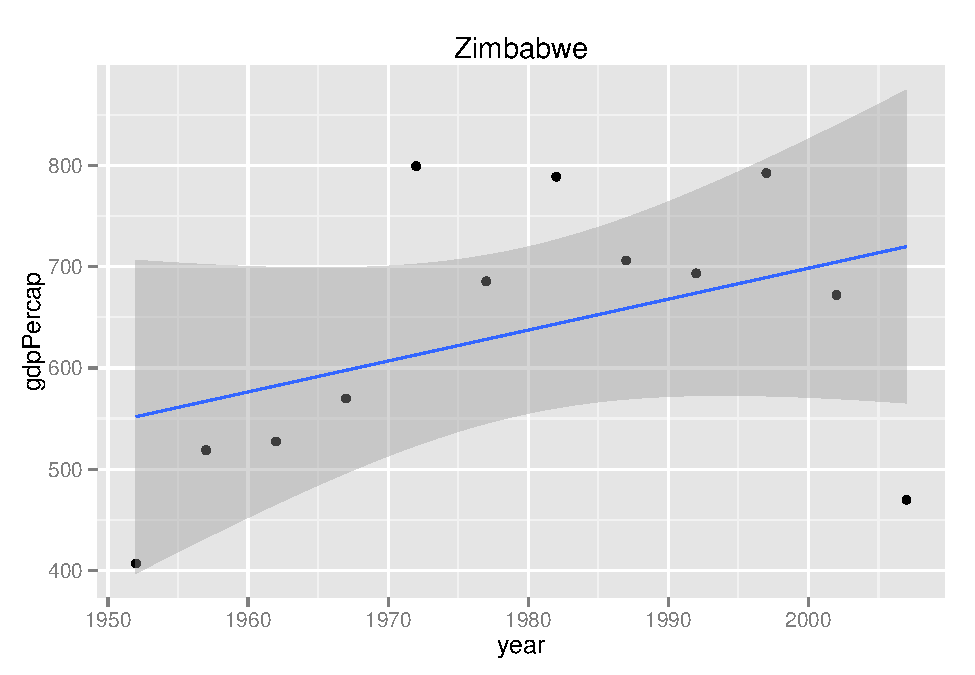
\includegraphics{GapMinder_rMarkdown_files/figure-latex/unnamed-chunk-3.pdf}

Summary stats by continent\ldots{} Buzzowga!

\begin{verbatim}
## 
## 
## |continent | MeanLifeExp| MinLifeExp| MaxLifeExp|
## |:---------|-----------:|----------:|----------:|
## |Africa    |       48.87|      23.60|      76.44|
## |Americas  |       64.66|      37.58|      80.65|
## |Asia      |       60.06|      28.80|      82.60|
## |Europe    |       71.90|      43.59|      81.76|
## |Oceania   |       74.33|      69.12|      81.23|
\end{verbatim}

Here is the global life expectancy. The second figure has really narrow
bin widths!

\begin{verbatim}
## stat_bin: binwidth defaulted to range/30. Use 'binwidth = x' to adjust this.
\end{verbatim}

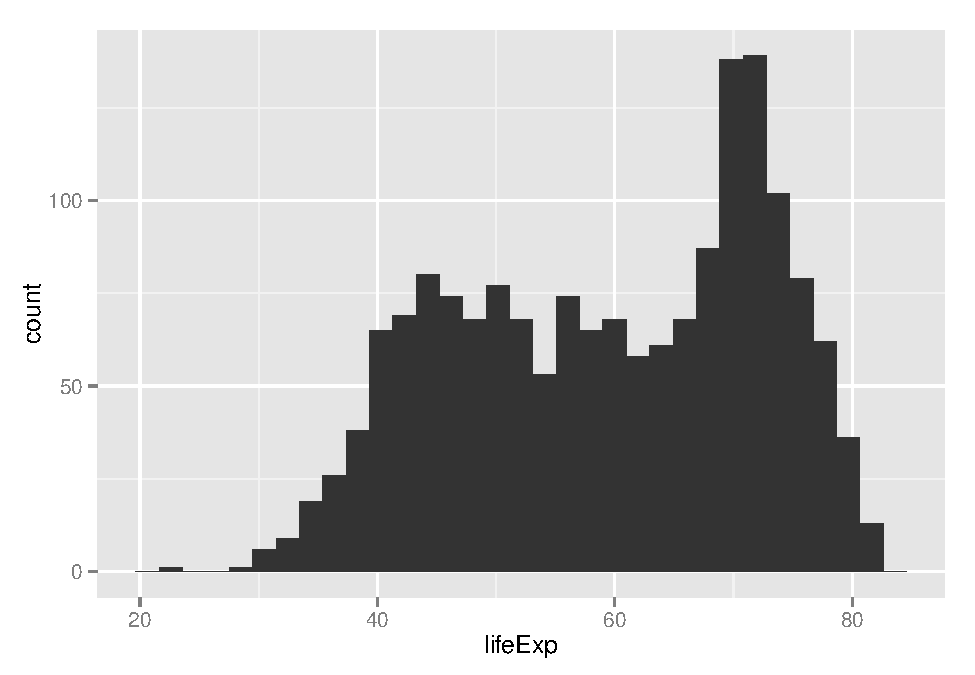
\includegraphics{GapMinder_rMarkdown_files/figure-latex/unnamed-chunk-41.pdf}
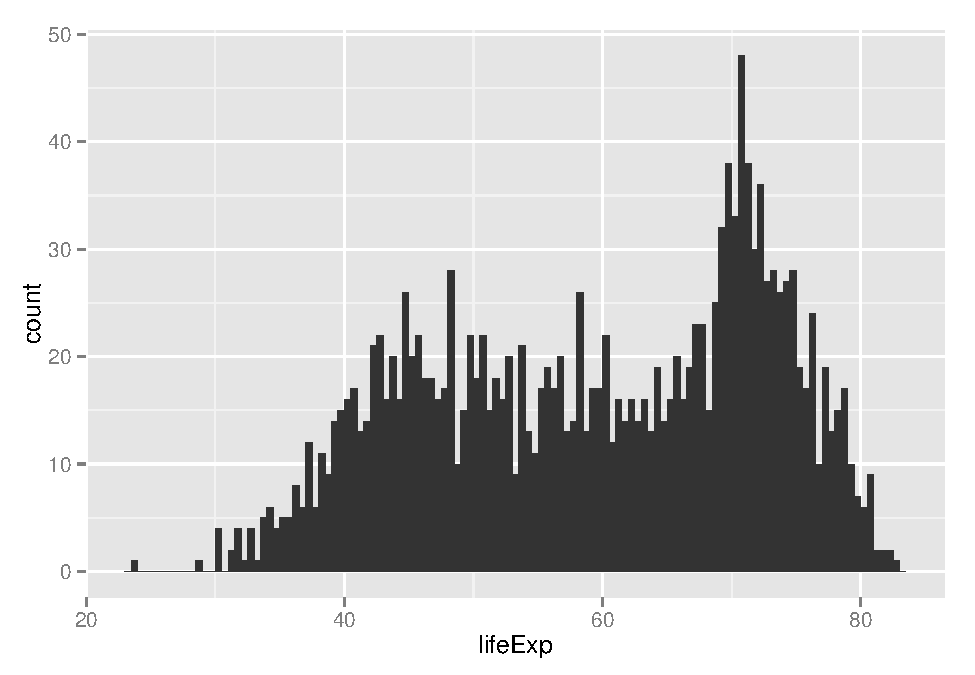
\includegraphics{GapMinder_rMarkdown_files/figure-latex/unnamed-chunk-42.pdf}

\end{document}
